\chapter{WLAN (Wireless Local Area Network)}
Bei einem drahtlosen Netzwerk findet die Übertragung ohne Kabel statt. Es werden elektromagnetische Wellen über die Luft übertragen. Für die drahtlose Übertragung im Netzwerk bedeutet dies, dass sich Layer 1 und Layer 2 ändern. Die darüber liegenden Layer bleiben unverändert. Durch diese Änderung der Übertragungsart ergeben sich einige Vorteile aber auch Nachteile.

\begin{table}[H]
	\begin{tabular}{l|l}
		\multicolumn{1}{c}{Vorteile} & \multicolumn{1}{c}{Nachteile} \\
		\hline
		+ BYOD: bring your own device & - Geteiltes Medium für viele Teilnehmen \\
		+ Kosten: Besonders in bestehenden Gebäuden & - Störungen \\
		+ Anpassungsfähigkeit & - Geschwindigkeit und Reichweite \\
		& - Security \\
	\end{tabular}
\end{table}

\textbf{Antennen} \\
Antennen sind die Grundlage für eine Übertragung über die Luft. Sie geben ein Signal in die Luft ab (Senderantenne) und können es auch wieder aus der Luft aufgreifen (Empfängerantenne). Je nach Anwendung eignen sich verschiedene Arten von Antennen.
\begin{itemize}
	\item Omnidirektionale Antennen: senden in alle Richtungen (Kugel)
	\item Direkte Antennen: Können gezielt senden
	\item MIMO (multiple input multiple output) Antennen: aktuell meist 8 Antennen
\end{itemize}

\textbf{Arten von Wireless Netzwerken} \\
Wie auch schon bei den verkabelten Netzen unterscheidet man Netzte nach ihrer Größe. Je nach Größe ergeben sich unterschiedliche Anforderungen und Schwierigkeiten.
\begin{itemize}
	\item WPAN: kurze Distanz (ca 10m), Frequenz meist 2.4 GHz z.B. Bluetooth, Zigbee
	\item WLAN: mittlere Distanz (ca 100m), Frequenz ist 2.4 GHz oder 5 GHz z.B. Wifi
	\item WMAN: große Distanz (kann sehr unterschiedlich sein), Frequenz zwischen 2 und 66 GHz z.B. Wifi, WiMax
	\item WWAN: riesige Distanzen (bis zu 50km), Frequenz zwischen 2 und 66 GHz z.B. WiMax
\end{itemize}

\textbf{Technologien von Wireless Netzwerken} \\
Es gibt unterschiedliche Technologien dir drahtlos übertragen. Je nach Reichweite und Anwendungsgebiete sind unterschiedliche Technologien sinnvoll. Nicht alle Technologien sind dazu geeignet oder dafür entworfen um Netzwerkdaten zu übertragen. Manche Technologien können dies trotzdem umsetzen.
\begin{itemize}
	\item Wifi (IEEE 802.11)
	\item Bluetooth (IEEE 802.15)
	\item WiMax (IEEE 802.16)
	\item Satelliten Breitband: kann als Internetzugang genutzt werden, z.B. Starlink (Oktober 2023 ca. 5000 Geräte, in einer Entfernung von 500 bis 600km, beantragt sind 22.000 Satelliten)
	\item Mobilfunk Breitband: viele verschiedene Standards die meist nach gravierenden Änderungen (Generationen) unterteilt werden. Bei der Änderung in eine neue Generation ist die Geschwindigkeit immer ein entscheidender Faktor (3G $\rightarrow$ 10x $\rightarrow$ 4G $\rightarrow$ 100x $\rightarrow$ 5G).
\end{itemize}

\section{Wifi (802.11)}
\textbf{Elektromagnetische Welle} \\
Gesendet wird mit elektromagnetischen Wellen. Diese kennt man vom sichtbaren Licht. Dort nimmt der Mensch unterschiedliche Wellenlängen als verschiedene Farben wahr. Jene Wellenlänge die zum übertragen von Wifi genutzt werden liegen außerhalb des sichtbaren Lichts. Dest länger die Welle ist, desto kürzer ist seine Frequenz (indirekt Proportional). Kurze Wellen besitzen mehr Energie als lange Wellen.
\begin{figure}[H]
	\centering
	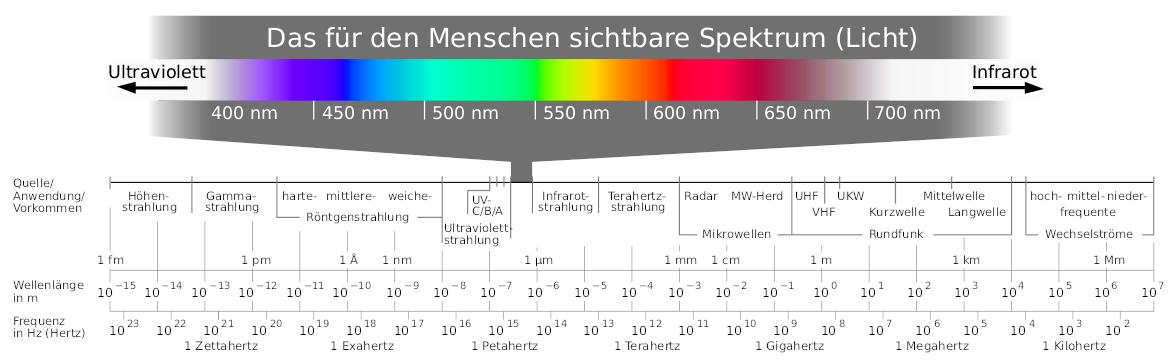
\includegraphics[width=1.0\linewidth]{figures/elektro_spektrum.png}
	\caption{Elektromagnetisches Spektrum}
\end{figure}
\begin{itemize}
	\item 2.4 GHz (1-10dm) UHF: Ultra High Frequency
	\item 5 GHz (1-10cm) SHF: Super High Frequency
\end{itemize}
Für das 5G Netz wurden neue Frequenzbereiche festgelegt und versteigert.
\begin{itemize}
	\item Mobilfunk: 600 MHz bis 6 GHz
	\item WLAN: 24 GHz bis 40 GHz
\end{itemize}

\textbf{Komponenten im WLAN}
\begin{itemize}
	\item Endgeräte: mit Netzwerkkarten und Antennen
	\item Wireless Router: Multifunktionsgeräte mit eingebautem Switch, Router, Modem Access Point,...
	\item Access Points: Schnittstelle zwischen dem drahtlosen Netz und dem verkabelten Netz. Man unterscheidet zwischen Autonomen-Access-Points (schwer erweiterbar) und Controller-Based-Access-Points.
\end{itemize}

\textbf{Wifi Frame} \\
\begin{tabular}{|l|l|l|}
	\hline
	Frame Control & Metainformationen z.B. Protokoll, Art des Frames,... & 2 Bytes \\
	\hline
	Duration & Übertragungsdauer, aufgrund unterschiedlicher Framelänge & 2 Bytes \\
	\hline
	Address 1 & Empfänger MAC-Adresse & 6 Bytes \\
	\hline
	Address 2 & Sender MAC-Adresse & 6 Bytes \\
	\hline
	Address 3 & MAC BSSID (WLAN Segment) & 6 Bytes \\
	\hline
	Sequence Control & Hängt vom AP ab &  \\
	\hline
	Address 4 & MAC-Adresse vom Access Point & 6 Bytes \\
	\hline
	Frame Body: & Header der restlichen Layer und Daten & \\
	\hline
	FC& Fehlerüberprüfung mit CRC & 4 Bytes \\
	\hline
\end{tabular}

\textbf{Operations-Modi}
\begin{itemize}
	\item Ad Hoc: Peer-to-Peer Netzwerk ohne Router
	\item Infrastruktur: Dahinter ein verkabeltes Netz
	\item Tethering: Hotspot zur Weiterleitung zwischen zwei Netzen 
\end{itemize}

\textbf{Kollisionen (CSMA/CA)} \\
Wireless Netzwerke nutzten eine Half Duplex Medium zum Senden. Man kann zeitgleich senden und empfangen. Zusätzlich ist es ein Shared Medium, das heißt viele Teilnehmer sind mit dem gleichem Medium verbunden. Somit kann es zu Kollisionen kommen (CSMA - Carrier Sense Multiple Access). Wifi löst das Problem mit Collision Avoidance (CA), es versucht also Kollisionen zu vermeiden. Falls gerade keiner sendet wird um Zeit beim Access Point angefragt. Dann erhält man einen Zeitslot indem man seine Daten senden und empfangen kann.

\textbf{Verbinden mit einem Accesspoint}
\begin{itemize}
	\item AP finden (aktiv, passiv)
	\item Authentifizieren: SSID, Passwort, Network Mode (a, b, g,...), Security (WPA, WPA2,...), Channel\\
	\item Verbindung herstellen
\end{itemize}

\textbf{Channels} \\
Die Frequenzen werden in kleinere Bereiche aufgesplittet. Gleiche Channels können sich gegenseitig stören. Überlappende Access Points sollten verschiedene Channels nutzen.
\begin{itemize}
	\item 2.4 GHz: Europa 13 Channels (1, 6 \& 11 nicht überlappend)
	\item 5 GHz: 24 Channels (alle ohne Überlappung)
\end{itemize}

\textbf{WLAN-Angriffe}
\begin{itemize}
	\item Datendiebstahl: Shared medium $\rightarrow$ Verschlüsselung
	\item DoS: falsch konfiguriert, Störsender,...
	\item Rogue Access Point: zusätzlichen falschen AP ins Netz eingefügt
	\item Evil Twin: einen AP einfügen, der gleich aussieht aber in ein anderes Netz führt
\end{itemize}

\textbf{Sicherheit und Verschlüsselung}
\begin{itemize}
	\item SSID Beacon verbergen (passic)
	\item MAC-Adressen filtern (L2 Security)
	\item Authentifizierung
	\begin{itemize}
		\item Open: ohne Password (nicht empfohlen)
		\item Shared Key: WEP, WPA (TKIP+AES), WPA2, WPA3
	\end{itemize}
\end{itemize}

Bei WPA2 unterscheidet zwei Varianten zum Authentifizieren:
\begin{itemize}
	\item Personal: ein Passwort für alles (PSK, Pre Shared Key), eher im privaten Bereich
	\item Enterprise: Anmeldung mit Username und Passwort, man meldet sich bei einem Server (z.B. RADIUS), eher im Firmenbereich
\end{itemize}

\textbf{WPA2-Personal Handshake: Pre-Shared-Key (4-Way)} \\
Zum Austausch der Schlüssel zwischen dem Access Point und dem Client findet ein 4-Way-Handshake statt. Dabei werden die benötigten Schlüssel generiert. Zum Generieren der Schlüssel muss das Passwort nie übertragen werden, deshalb nennt man die Variante auch PSK (Pre-Shared-Key). Der Schlüssel wurde also davor schon ausgemacht.

\begin{figure}[H]
	\centering
	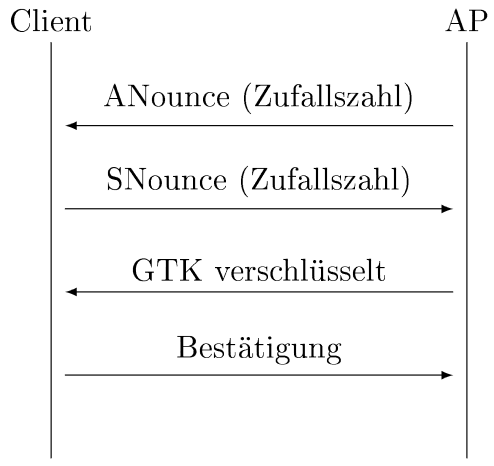
\includegraphics[width=1.0\linewidth]{figures/wpa2_personal_handshake.png}
	\caption{WPA2 Personal Handshake}
\end{figure}
PTK (Pairwise Transient Key): für Unicasts, jeder hat seinen eigenen Schlüssel mit dem AP \\
PTK = PRF(Pwd+ANounce+SNounce+APMAC+ClientMAC) \\
PRF (Pseudo Random Function): ist eine Pseudo-Zufallsfunktion die dann den Schlüssel erzeugt und den Geräten bekannt ist. \\
GTK (Group Temporal Key): für Broadcast und Multicasts im Netz, für alle Teilnehmer gleich. \\

Das Passwort wird nie über das Medium ausgetauscht, deshalb nennt man das Verfahren Pre Shared Key. Die Nachricht wird nach Layer 2 verschlüsselt. Dieser kann nicht verschlüsselt werden, da der Access Point die Frames identifizieren muss. Danach im verkabelten Netz, wie sonst auch immer, wird wieder nach Layer 4 verschlüsselt (z.B. mit TLS).